\chapter{基于解的局部性的自适应优化方法}
在上一章中,我们发现了延迟数据一致性方法的性能提升的相对大小和冗余计算的比例有关。
为了得到更好的性能提升,延迟数据一致性方法需要尽可能的避免冗余计算。
在本章中,从如何降低冗余计算比例这一问题出发,本课题最终实现了基于解的局部性这一自适应优化方法。
在这一方法指导的开启策略下,延迟数据一致性方法获得了相对最优的性能提升。

在本章中,我们先是从单个顶点的角度出发分析了全局解和局部解的局部性关系有利于减少冗余计算。
然后通过实验对图计算过程中全体活跃点上全局解和局部解的关系进行了分析,发现了解的局部性这一规律。
从这一规律入手,通过在线统计的方法,本课题最终实现了基于解的局部性的自适应优化方法。
最后,本章在不同图算法和输入图的组合上对这种方法进行了评测,验证了它的性能提升效果。

\section{全解解和局部解如何影响冗余计算}

在分布式图计算中,由于副本点的存在,每个顶点上的全局解由多个局部解构成。
在把图计算迭代公式改写为差值累加的形式之后,图计算通过交换构成局部解的消息累加值来实现不同副本点上的全局解的一致。

当顶点上的全局解由多个局部解构成时,那么多个局部解都不等于全局解。
那么用这样的局部解进行的本地计算自然是冗余无效的。
当顶点上的全局解由单个局部解构成时,那么这个局部解就等于全局解。
用已经等于全局解的局部解进行本地计算自然是有效的。
同时由于其他副本上没有局部解,副本点就不记录为活跃点,也就不会产生本地计算。
这些副本会在数据一致时收到消息,从而得到和全局解一致的视图。
也就是说就单个顶点而言,全局解由多个局部解构成时不利于开启延迟数据一致性方法,
全局解由单个局部解构成时有利于开启延迟数据一致性方法。


在图\ref{fig:useless_and_local}中,我们再次以 sssp 为例子直观的展示全局解和局部解如何影响冗余计算。
图\ref{fig:useless_and_local}中,左侧给出了一个全局解由多个局部解构成的例子,右侧给出了一个全局解由单个局部解构成的例子。
在左侧中,一个顶点在5台机器上分布着副本点,并且5台机器上分别存在着6,7,7,8,9着5个局部解。
根据sssp中对局部解之间$\oplus$的定义:$a\oplus b=std::min(a,b)$,全局解为6。
所以只有一个局部解等于全局解,在机器1,2,3,4上的局部解都不等于全局解。
如果此时对这5个副本点使用延迟数据一致性方法,那么机器1,2,3,4上的副本点所进行的本地计算都是无效而冗余的。
在右侧中,同样是一个顶点在5台机器上分布着副本点,但是只在机器2上存在局部解,此时机器2上的局部解就是全局解。
如果此时对这5个副本使用延迟数据一致性方法,那么机器0,1,3,4上的副本由于没有收到消息不被激活,所以不产生本地计算。
机器2上的副本其局部解就等于全局解,所以机器2上所进行的本地计算是有效的。
在数据一致性时,机器0,1,3,4上的副本会通过消息交换得到和机器2上的副本同样的全局视图。



\begin{figure}[!htbp]
\centering
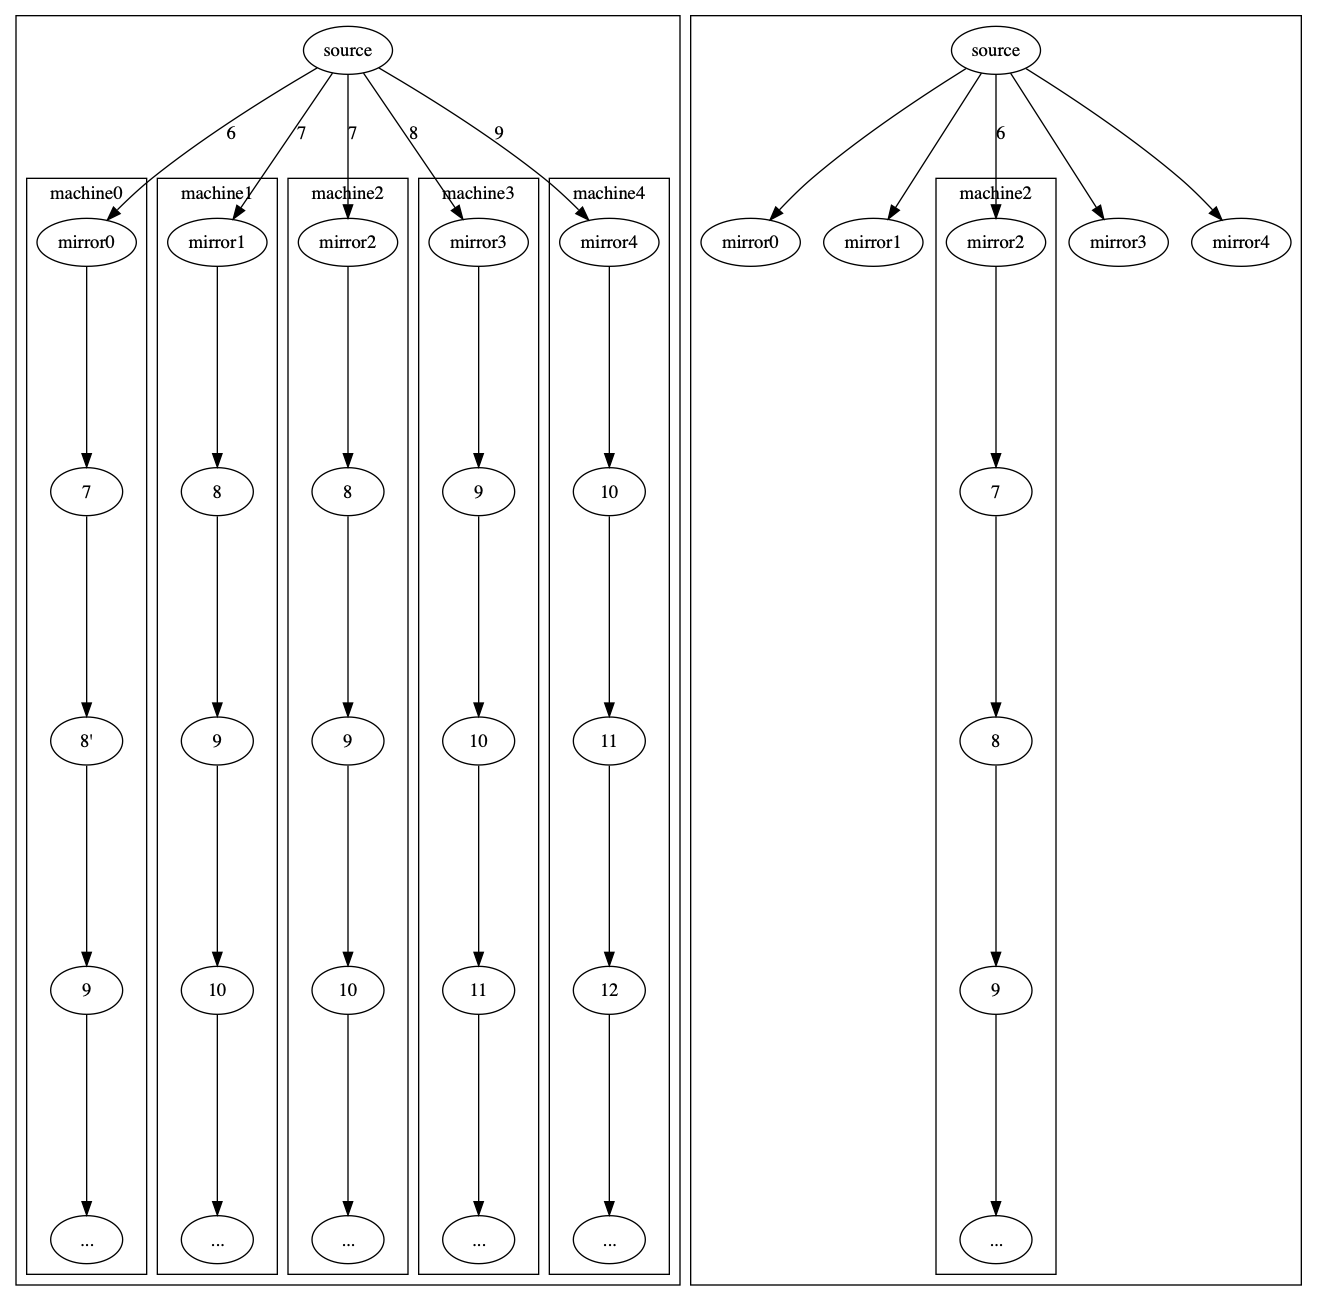
\includegraphics[width=0.8\textwidth]{useless_and_local}
\bicaption{解的局部性如何影响冗余计算}{How the locality of the solution affects redundant calculations}
\label{fig:useless_and_local}
\end{figure}


通过上边的例子我们可以看到,全局解由单个局部解构成时有利于开启延迟数据一致性。
在图计算过程中的任何时刻,全局解由单个局部解构成和由多个局部解构成的情况都是同时存在的。
但是如果大多数顶点的全局解都只由当局部解构成,那么此时显然是开启延迟数据一致性的良好时机。
这种情况我么称之为解的局部性。

\section{全局解和局部解的关系中的局部性规律}
为了研究图计算过程中解的局部性的变化规律,我们需要保存每次迭代过程中的局部解,然后对其进行观察。

在图计算过程中,局部解由本地的消息累加和构成。
这些消息累加和被包含在消息中然后在集群结点之间进行交换。
消息交换在图计算中起着重要作用,消息中的消息累加和承载了下一轮迭代有哪些活跃点以及这些活跃点收到的消息这些重要信息。
当消息为空时,系统中没有活跃点,图计算也就收敛结束了。

在m2m方式的消息交换中,系统通过三个阶段完成副本点之间的局部解的交换从而实现数据一致。
第一个阶段,所有的副本点向 master 点发送自己的消息累加和。
master 点收到所有副本点上的消息累加和之后按照事先定义的$\oplus$操作符对这些消息累加得到全局消息累加和。
此时进入第二个阶段,master 点向所有副本点发送全局消息累加和。
此时所有的副本点都得到了一份原有的本地消息和全局消息累加和。
由于全局消息累加和中存在着重复的本地消息,所以消息交换还需要第三个阶段,
每个副本点要在全局消息累加和中减去自己的本地消息。
最终经历这三个阶段,每个副本点都得到了相同的消息累加和从而得到相同的全局视图。


可以看到局部解直接体现为副本点的本地消息累加和。
但是图计算过程中并不关心副本点上的消息累加和之间的数量和相对数值,只关心最终的全局消息累加和。
消息交换完成得到全局消息累加和之后,代表着局部解的本地消息累加和就会被清空。
所以,为了记录局部解和全局解从而分析它们的规律,我们需要给 vertex data 添加两个数据结构。
一个是$std::map<int,T> data\_at\_iter$用于记录第$i$次迭代时顶点的全局解。
一个是$std:map<int, std::vector<message\_type>> local\_sum$用于记录第$i$次迭代时
顶点收到的多个消息累加和。

在顶点进行全局的 apply 操作时,系统可以在顶点上记录下全局解。
为了记录消息累加和则需要在两个地方添加代码。
第一处是master点发送自己的本地消息累加和,由于不通过网络交换消息,这里可以直接写入。
第二处是为了记录mirror点向master点通过网络发送的本地消息累加和,需要在收消息的地方添加代码。
通过以上两个地方添加记录消息累加和的代码,保证了对局部解的记录是不重不漏的。 
需要说明的是,局部解的数量有可能少于副本点的数量。
因为那些不被激活的副本点是不会向 master 发送包含本地消息累加和的消息的。


图\ref{fig:local_sssp}给出了一个具体的顶点上记录到的全局解和消息累加和的例子。
图中第一列是顶点id,第二列是最终解,第三列是迭代解,第四列是副本点的数据,接下来是顶点上收到的多个消息累加和,
最后一列是顶点上一轮的迭代解。
以图中3629703号顶点为例,可以看到这个顶点有20个副本,全局解是6,由15个局部解构成,并且其中7个局部解都不等于全局解。
在这样的顶点上使用延迟数据一致性方法显然会造成一定数量的冗余计算。
而以图中411911号顶点为例,可以看到这个顶点也有20个副本,全局解是7,但是只由一个局部解构成。
那么像这样的顶点显然是存在着解的局部性的,使用延迟数据一致性方法不太容易造成冗余计算。


\begin{figure}[!htbp]
  \centering
  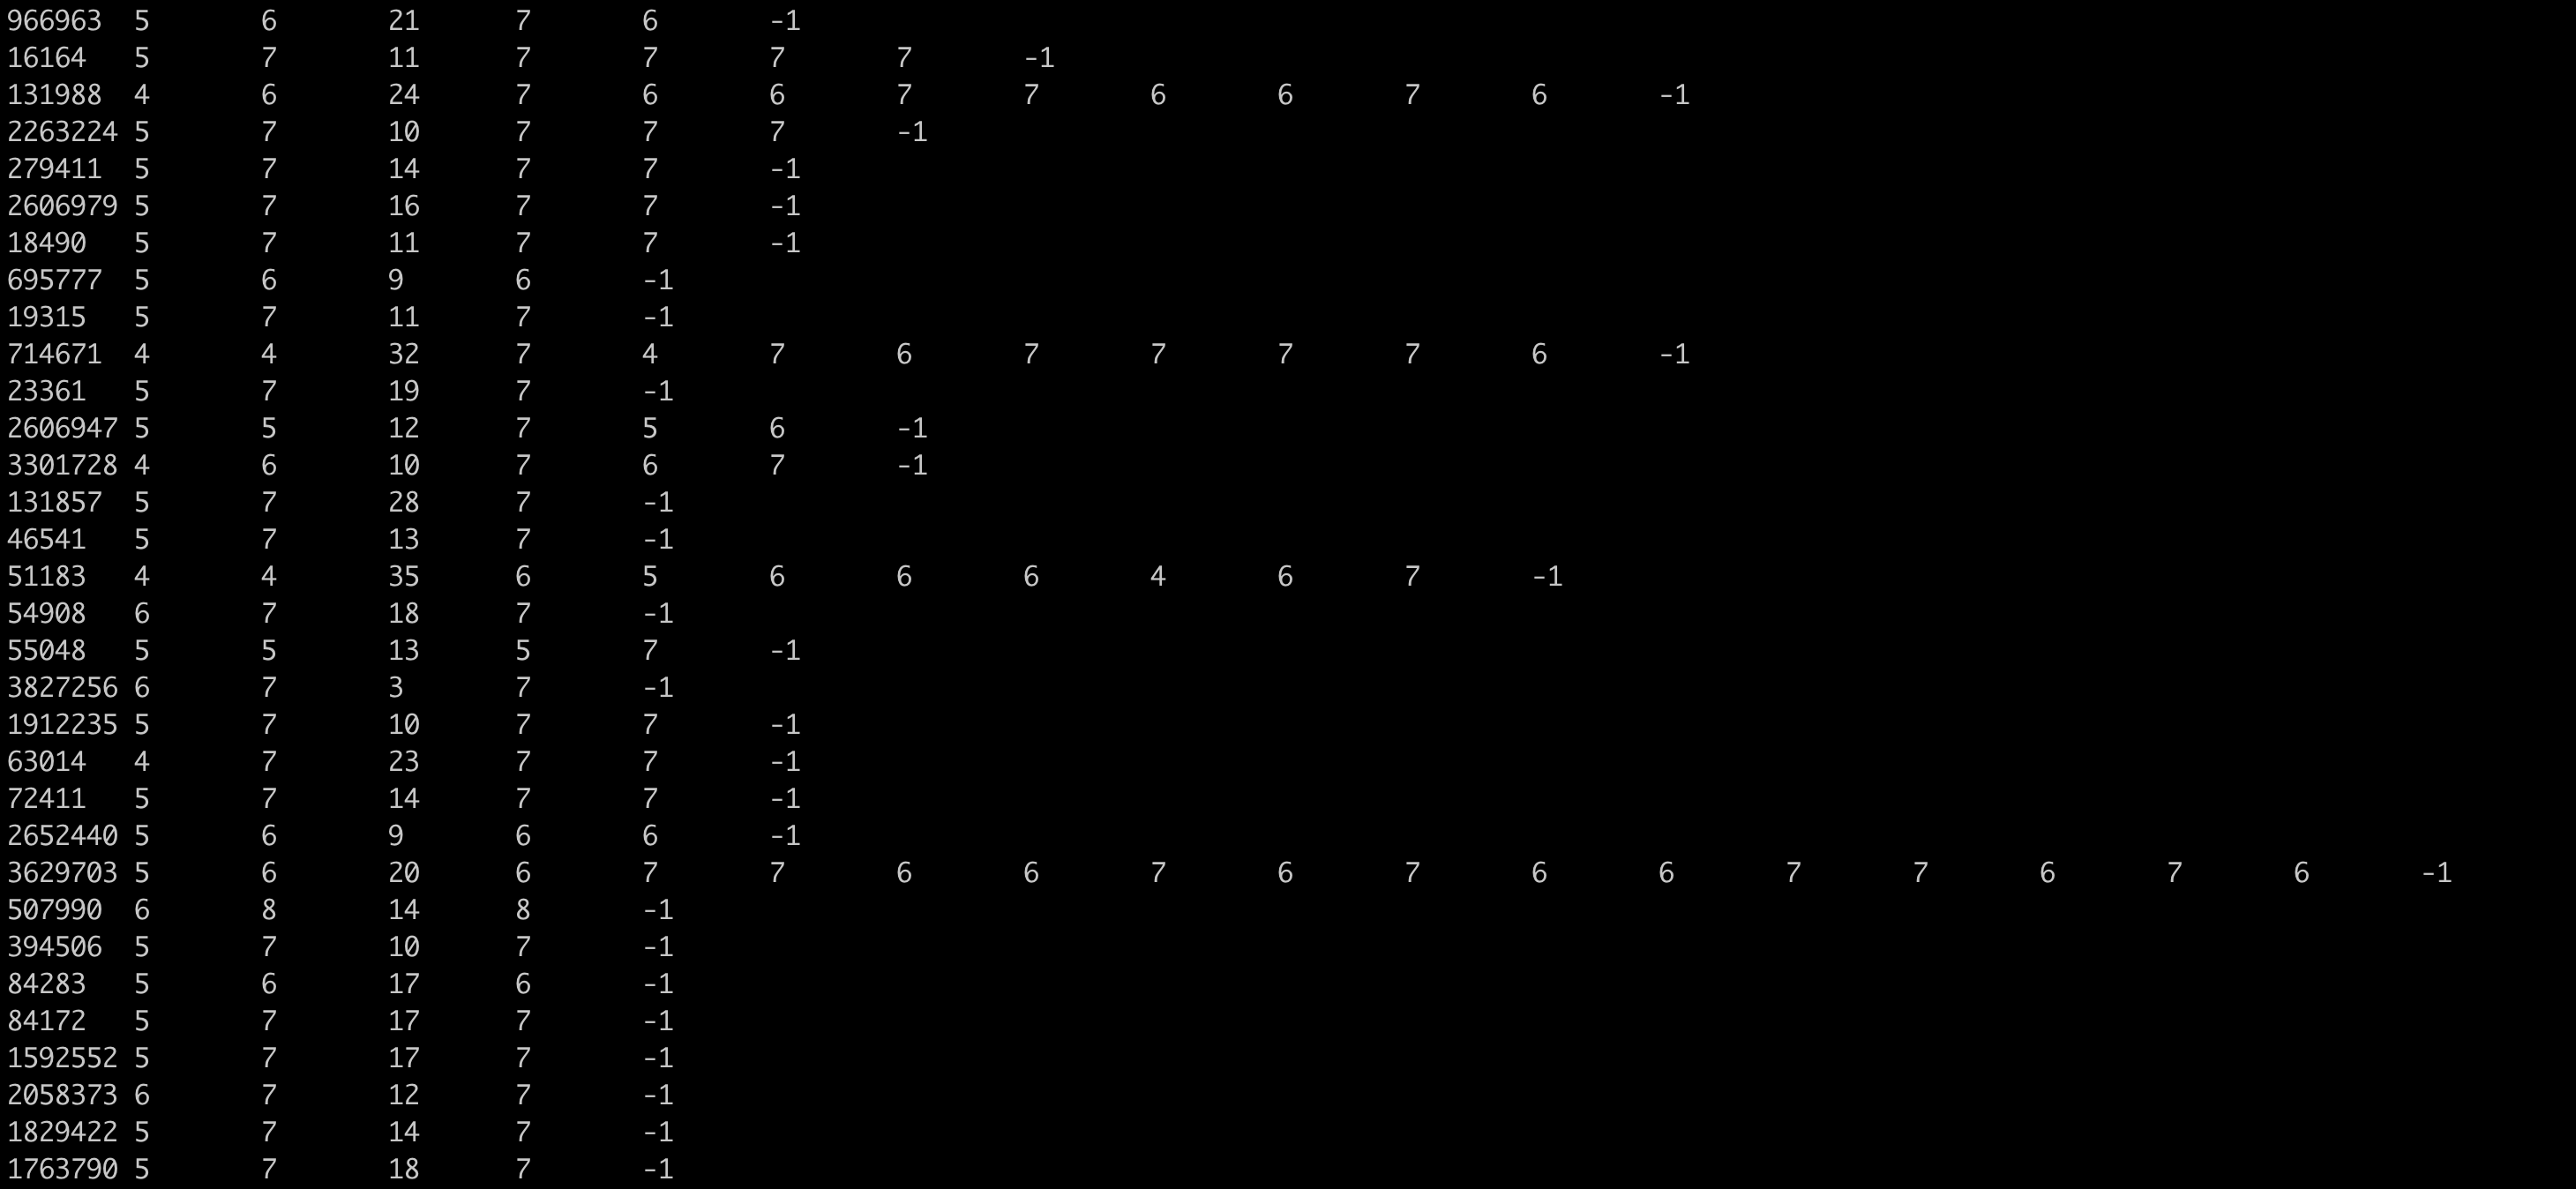
\includegraphics[width=0.8\textwidth]{local_sssp}
  \bicaption{局部解示意图}{Local solution diagram}
  \label{fig:local_sssp}
\end{figure}
%用mapreduce进行统计
通过记录具体的本地消息累加和,我们可以观察在迭代过程中解的局部性的变换规律。
即图计算的迭代过程中,有多少顶点上的全局解是由单个局部解构成的,这样的顶点是否占多数。
图计算完成之后,运行时记录的全局解和局部解这些信息保存在了 graph 中。 
利用 PowerGraph 提供的 map-reduce 接口,我们可以通过 graph 上记录的数据具体统计每一轮迭代中
全局解由多个和单个局部解构成的顶点的数量。

%统计结果

通过在计算引擎中添加代码和使用map-reduce接口进行统计,本课题在4种常用的图算法和8个典型的图上得到了以下的实验结果。

通过分析我们可以看到,在4种算法和输入图上,在图计算的后期都存在着典型的解的局部性规律。
即在每轮的活跃点中,大部分顶点的全局解都只由单个局部解构成,由多个局部解构成全局解的顶点只占极少数,甚至没有。
但是在图计算的前期,解的局部性的变化规律则和具体的算法,输入图,以及集群配置有关。


在有些图上,由多个局部解构成全局解的点从一开始就只占极少数,并且数量一直在下降。
而在有些图上,由多个局部解构成全局解的点则存在一个先上升后下降的趋势。
也就是说,解的局部性在有的图和算法的组合上是一直都存在的。
而在另外一些图和算法的组合上,则是随着迭代的进行才逐渐出现。

同时结合之前的决策树策略来分析,我们发现它们在开启策略的选择上是一致的。
在决策树策略中,针对那些 $e\_div\_v$ 小于 10 的图,系统直接开启延迟数据一致性方法,就能获得相对较好的性能提升。
而在我们的实验中发现,那写 $e\_div\_v$ 小于 10 的图,确实一开始就存在着解的局部性的规律。
针对那些 $e\_div\_v$ 大于 10 的图, 决策树指导系统在活跃点下降率超过7\%时开启延迟数据一致性方法,然后就能获得相对较好的性能提升。
而在我们的实验中发现,活跃点下降超过7\%的时间节点,也是那些 $e\_div\_v$ 大于10的图开始出现解的局部性的规律的时候。

% 同时对于决策树失灵的情况
%结果分析

\section{基于解的局部性的自适应优化方法}
在上一节中,我们通过实验证明了在图计算过程中确实存在着解的局部性规律。
解的局部性这种规律和具体的输入图及算法有关,在迭代的某个时间节点之后才存在。
通过统计全局解由多个局部解构成的顶点的数量,我们可以观察和判断出解的局部性。


延迟数据一致性方法的性能提升受冗余计算的影响。而解的局部性则可以用于减少冗余计算。
基于此,我们最终提出了一种基于解的局部性的自适应优化方法,它指导延迟数据一致性方法
在图计算开始出现的解的局部性的时候来开启延迟数据一致。

在之前的实验中,我们通过保存局部解的方式在图计算完成之后对迭代过程中解的局部性进行观察。
这种事后离线实验的方式只能帮助我们观察图计算过程中的规律,却无法直接作为开启策略。
为了实现基于解的局部性的自适应优化方法,我们需要找到一种在线的统计方式。

在之前的实验中,为了观察局部解的具体数量和数值,我们需要对本地累加和进行记录保存。
但是如果只是为了统计全局解由多个局部解构成的顶点的数量,我们并不需要记录保存本地累加和。
分析消息交换的过程我们发现,只需要在消息交换的过程增加一些判断条件,
我们就能实现在线地统计全局解由多个局部解构成的顶点的数量这一目的。

实现了在线即时统计全局解由多个局部解构成的顶点的数量这一目的之后,
我们就真正的得到了一个基于解的局部性的自适应优化方法。
这种方法克服了决策树策略需要事先大量手动调优,并且存在过拟合现象这些缺点。

\section{性能评测}

% \section{本章小结}